\documentclass[english, 11pt]{article}
\usepackage{../notes}

\newcommand{\thiscoursecode}{PHYS 234}
\newcommand{\thiscoursename}{Quantum Physics I}
\newcommand{\thisprof}{Dr. Robert Hill}
\newcommand{\me}{Liam Horne}
\newcommand{\thisterm}{Spring 2014}
\newcommand{\website}{LIHORNE.COM}

% Headers
\chead{\thiscoursename}
\lhead{\thisterm}

%%%%% TITLE %%%%%
\newcommand{\notefront} {
\pagenumbering{roman}
\begin{center}

{\ttfamily \url{\website}} {\small}

\textbf{\Huge{\noun{\thiscoursecode}}}{\Huge \par}

{\Large{\noun{\thiscoursename}}}\\ \vspace{0.1in}

\vspace{0in}
\includegraphics[scale=0.5]{../logo.png}

  %\includegraphics[scale=0.1]{shield.png} \\
  {\noun \thisprof} \ $\bullet$ \ {\noun \thisterm} \ $\bullet$ \ {\noun {University of Waterloo}} \\

  \end{center}
  }

%   ooooo      ooo   .oooooo.   ooooooooooooo oooooooooooo  .oooooo..o
%   `888b.     `8'  d8P'  `Y8b  8'   888   `8 `888'     `8 d8P'    `Y8
%    8 `88b.    8  888      888      888       888         Y88bo.
%    8   `88b.  8  888      888      888       888oooo8     `"Y8888o.
%    8     `88b.8  888      888      888       888    "         `"Y88b
%    8       `888  `88b    d88'      888       888       o oo     .d8P
%   o8o        `8   `Y8bood8P'      o888o     o888ooooood8 8""88888P'

\begin{document}

  % Notes fron
  \notefront
  % Table of Contents and List of Figures
  \tocandfigures
  % Abstract
  \doabstract{These notes are intended as a resource for myself; past, present, or future students of this course, and anyone interested in the material. The goal is to provide an end-to-end resource that covers all material discussed in the course displayed in an organized manner. If you spot any errors or would like to contribute, please contact me directly. \\}

  Robert Hill is a low temperature experimentalist, but this course will be mostly theoretical.
  \newline

   Albert Einstein once said, "Quantum mechanics is certainly imposing. But an inner voice tells me that it is not yet the realthing. The theory says a lot, but does not really bring us any closer to the secret of the 'old one'. I, at any rate, am convinced that He does not throw dice."
   \newline

   Richard Feynman said "I think I can safely say that nobody understand quantum mechanics."
   \newline

   So we're in for miserable experience with this course then? Well not really, there are some good reasons to study Quantum Physics:

   \begin{itemize}
     \item It's Extremely interesting!
     \begin{itemize}
        \item Physically
        \item Mathematically
        \item Philosophically
      \end{itemize}
      \item It is the science behind future technology!
      \item Waterloo is Quantum Valley!
   \end{itemize}

   \section{The Photoelectric and Compton Effects}

     \subsection{Historical Background}
       In classical physics we always observed things as behaving like waves or as particles. For example, there is

       \begin{itemize}
         \item Particle-like behaviour of radiation
         \item Wave-like behaviour of matter
         \item Wave-particle duality that combines the two
       \end{itemize}

       Let's explore the two sides of the coin. First, {\bf what is a particle?} Some words that describe it are {\textit point, localised, mass, solid} and similarly {\bf what is a wave?} It can be described with words like \textit{interference, oscillation, delocalised}, and \textit{medium}. One such thing that we have had trouble with describing is {\bf light}. Is it a wave or a particle?

     \subsection{Einstein's Theory of Photoelectric Effect}

       Radiant energy (light) is quantized into concentrated bundles (photons)

       \[ E = hf \]

       His Photoelectric Equation (1905) states that

       \[ K_{\mbox{max}} = hf - \omega_0 \]

     \subsection{Compton Effect}

       In the photoelectric effect, we treated light as being composed of individual light particles, called photons, that carry some energy. It then makes sense to think that the photons also have momentum.
       \newline

       Electromagnetic radiation is scattered by a target object. In classical theory, the charges in the target object will respond to the incoming wave and start to oscillate. All oscillating charges emit radiation at the frequency of oscillation, and this newly generated set of waves can also be detected at an angle θ with respect to the incoming wave. This classical model explains why the sky is blue and all that jazz. The scattering process itself, though, does not change the frequency of incoming and outgoing radiation.
       \newline

       However, an experimental problem occurred. In experiments with X-ray radiation on a graphene target, one observes that two separate frequencies at an angle $\theta$ result in different intensities. This effect is independent of the material, though intensities may vary.
       \newline

       \begin{defn}[Compton Shift]\label{compton_shift}
         \[ \Delta \lambda = \lambda_c (1 - \cos \theta) \]
       \end{defn}

       \begin{defn}[Compton wavelength]\label{compton_wavelength}
         \[ \lambda_c = \f{h}{m_0c} \]
       \end{defn}

       \begin{figure}[t]
         \centering
           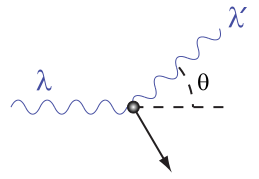
\includegraphics[width=0.35\textwidth]{compton_scattering.png}
         \caption{The Compton Effect. The scattered light has a different frequency; the frequency depends on the direction. A bigger deflection causes a bigger change in frequency.}
       \end{figure}

   \section{De Broglie Wavelength and the Davisson-Germer Experiement}

     We have shown that wave phenomena can exhibit particle features. We can rewrite the momentum instead as $p = \f{h}{\lambda}$ using a simple wave relationship. There is nothing in this reformed equation that has to do with light. This led to the following postulate.

     \subsection{The De Broglie Postulate (1924)}
       De Broglie's hypothesis was based on the grand symmetry of nature; if radiation has wave-particle duality, then so should matter.
       \begin{defn}[de Broglie Relation]\label{de_broglie_relation}
         \[ \lambda = \f{h}{p} \]
       \end{defn}

     \subsection{The Davisson-Germer Experiment}
       We must first understand the Bragg Grating; it is an optical filter that re- flects particular wavelengths and transmits all others. Note that reflection, however, is common to both waves and particles.


  \end{document}
